\section{度量与度量空间}
\label{sec:metric-definition}

实数之间用绝对值比较远近，向量之间用范数比较远近，二进制串之间可以数有多少位不同，图中两个顶点之间可以数最少要走几条边。这些比较方法的对象和计算方式各不相同，却共同遵守几条规则。本节先把这些规则提炼为度量的定义，再列出常见度量，最后研究在只看一部分对象、组合多个对象或忽略部分差异时，怎样从已有度量得到新的度量。

\subsection{度量的定义}
\label{sec:metric-axioms}

在实轴上，$|x-y|$不取负值，只在$x=y$时为零，与两数的先后无关，并且满足$|x-z|\leq|x-y|+|y-z|$。平面上的欧氏距离也具有这四条性质。后面关于邻近、收敛和连续的论证只用到这四条性质，因此把它们取为定义。

\begin{definition}[度量与度量空间]
\label{def:metric-space}
设$X$是非空集合。若函数$d:X\times X\to[0,\infty)$对任意$x,y,z\in X$满足
\begin{enumerate}
  \item 分离性：$d(x,y)=0$当且仅当$x=y$；
  \item 对称性：$d(x,y)=d(y,x)$；
  \item 三角不等式：$d(x,z)\leq d(x,y)+d(y,z)$，
\end{enumerate}
就称$d$为$X$上的一个\term{度量}（metric），也称距离函数；称$(X,d)$为\term{度量空间}（metric space），$d(x,y)$称为$x$与$y$之间的距离。
\end{definition}

陪域取为$[0,\infty)$已经包含了非负性，并且要求距离总是有限的实数。这四条要求各自排除一种不合适的比较方式。非负性排除了“负的远近”；分离性要求不同的点距离严格为正，比较规则能够辨认不同对象；对称性要求从$x$看$y$与从$y$看$x$得到同一个数。三角不等式最为关键：经过中间点$y$绕行的总长度，不会短于直接从$x$到$z$的距离。正因为如此，一段难以直接估计的距离可以拆成几段容易估计的距离再相加。

\paragraph{反向三角不等式}
三角不等式给出距离之和的上界；后面的极限估计还常常需要两个距离之差的上界。对任意$x,y,z\in X$，三角不等式给出$d(x,z)\leq d(x,y)+d(y,z)$，即$d(x,z)-d(y,z)\leq d(x,y)$；交换$x$与$y$的角色，又得到$d(y,z)-d(x,z)\leq d(x,y)$。两式合起来就是
\begin{equation}
\label{eq:metric-reverse-triangle}
  \bigl|d(x,z)-d(y,z)\bigr|\leq d(x,y).
\end{equation}
它说明：把比较点从$x$移动到$y$，到固定点$z$的距离至多改变$d(x,y)$。图~\ref{fig:metric-triangle}把两种不等式画在同一个三角形中。

\begin{figure}[!htbp]
  \centering
  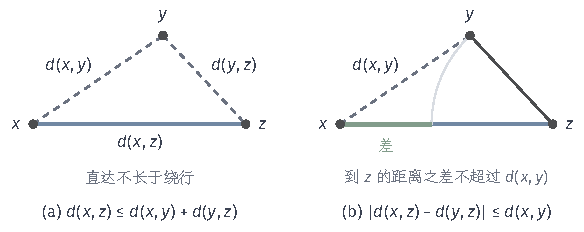
\includegraphics[width=98.972mm]{figures/02-abstract-mathematics/01-metric-and-measure/tikz/c1-triangle-inequality/figure.pdf}
  \caption{三角不等式与反向三角不等式。(a) 从$x$到$z$的直达距离（蓝色实线）不超过经中间点$y$的绕行长度（灰色虚线）。(b) 把比较点从$x$移到$y$时，到固定点$z$的两段距离之差（绿色标出的长度差）不超过移动的距离$d(x,y)$。}
  \label{fig:metric-triangle}
\end{figure}

\paragraph{集合与度量一起给出}
同一个集合可以配备不同的度量，所以度量空间是集合与度量组成的对，而不是集合本身。例如在$\mathbb R$上，除了通常距离$|x-y|$，还可以取下一小节的离散距离：任意两个不同的数距离都是$1$。在通常距离下，$1/n$与$0$的距离$1/n$越来越小；在离散距离下，这个距离始终是$1$。因此“$1/n$是否接近$0$”没有脱离度量的答案。后面凡是谈到邻近、收敛和连续，都要先说明使用的是哪个度量；在不致混淆时，才把$(X,d)$简称为$X$。

\subsection{常见度量}
\label{sec:metric-examples}

最常见的度量来自向量的范数；但度量并不要求对象能做减法，计数和路径长度同样可以给出度量。

\paragraph{由范数诱导的度量}
设$\lVert\cdot\rVert$是$\mathbb R^d$上的一个范数，即满足正定性、正齐次性$\lVert c\bm x\rVert=|c|\,\lVert\bm x\rVert$与三角不等式$\lVert\bm x+\bm y\rVert\leq\lVert\bm x\rVert+\lVert\bm y\rVert$的非负函数；常用的$\ell^1$、欧氏和最大值范数及其性质见\BookChapterRef{chap:normed-inner-product-spaces}{卷一“赋范空间与内积空间”章}。令$d(\bm x,\bm y)=\lVert\bm x-\bm y\rVert$，度量的三条要求逐条来自范数公理：正定性给出$d(\bm x,\bm y)=0\Leftrightarrow\bm x-\bm y=\bm 0$；取$c=-1$得到$\lVert\bm y-\bm x\rVert=\lVert\bm x-\bm y\rVert$，即对称性；把$\bm x-\bm z$写成$(\bm x-\bm y)+(\bm y-\bm z)$再用范数三角不等式，就得到度量的三角不等式。三种常用范数给出
\[
  \begin{aligned}
    d_1(\bm x,\bm y)&=\sum_{i=1}^d|x_i-y_i|,\qquad
    d_2(\bm x,\bm y)=\Bigl(\sum_{i=1}^d|x_i-y_i|^2\Bigr)^{1/2},\\
    d_\infty(\bm x,\bm y)&=\max_{1\leq i\leq d}|x_i-y_i|.
  \end{aligned}
\]
$d_1$把各坐标的偏差全部累加，$d_\infty$只记录最大的一个坐标偏差，$d_2$介于两者之间。

\begin{example}[同一组点的三种距离]
\label{ex:metric-three-distances}
在$\mathbb R^2$中取$\bm p=(0,0)$、$\bm q=(4,0)$、$\bm r=(3,3)$。$\bm q-\bm p=(4,0)$只有一个坐标偏差，三种距离都等于$4$。$\bm r-\bm p=(3,3)$的偏差分在两个坐标上，于是
\[
  d_1(\bm p,\bm r)=6,\qquad d_2(\bm p,\bm r)=3\sqrt2\approx4.243,\qquad d_\infty(\bm p,\bm r)=3.
\]
在$d_1$和$d_2$下$\bm q$离$\bm p$更近，在$d_\infty$下却是$\bm r$更近。图~\ref{fig:metric-three-distances}画出了三种读数：$d_1$沿坐标方向折线累加，$d_2$取直线段，$d_\infty$只看较长的那条坐标边。哪个点“更近”取决于我们怎样累计各坐标上的偏差。
\end{example}

\begin{figure}[!htbp]
  \centering
  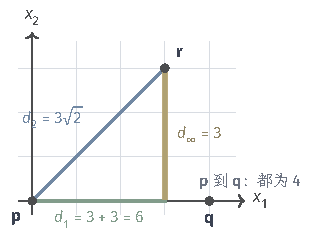
\includegraphics[width=52.871mm]{figures/02-abstract-mathematics/01-metric-and-measure/tikz/c1-three-distances/figure.pdf}
  \caption{同一组平面点在三种度量下的距离。$\bm q$与$\bm p$只在横坐标上相差$4$，三种距离都是$4$；$\bm r$与$\bm p$在两个坐标上各差$3$，$d_1$按折线累加得$6$，$d_2$取直线长度$3\sqrt2$，$d_\infty$只取较大的坐标差$3$。}
  \label{fig:metric-three-distances}
\end{figure}

\paragraph{不需要减法的度量}
在任意非空集合$X$上令$d(x,y)=0$（$x=y$）、$d(x,y)=1$（$x\neq y$），得到\term{离散度量}（discrete metric）。前两条要求直接由定义成立；对三角不等式，若$x=z$，左边为$0$；若$x\neq z$，则$y$不可能同时等于$x$和$z$，右边至少有一项为$1$。离散度量只回答“相同或不同”，不衡量差别大小，常用来构造反例。

对长度为$m$的两个二进制串$x=x_1\cdots x_m$与$y=y_1\cdots y_m$，\term{Hamming距离}（Hamming distance）定义为不同位置的个数$d_H(x,y)=\#\{i:x_i\neq y_i\}$，其中$\#$表示集合的元素个数。例如$d_H(10110,11100)=2$，两串在第2、4位不同。三角不等式逐位检查：若$x_i\neq z_i$，则$x_i\neq y_i$与$y_i\neq z_i$至少有一个成立，所以$x$与$z$不同的位置都被计入右边两项中的至少一项。这里用的是逐坐标比较，而不是对串做减法。

设$\mathcal G=(V,E)$是无权、无向的连通图，令$d_{\mathcal G}(u,v)$为从$u$到$v$的路径所含边数的最小值，即\term{最短路距离}（shortest-path distance）；最短路的计算见\BookChapterRef{chap:graph-optimization}{卷一“图上的组合优化”章}。连通性保证每对顶点之间都有路径，最小值是有限的非负整数；分离性来自“长度为零的路径只能停在原地”，对称性来自无向图中路径可以反向走。三角不等式靠路径拼接：把$u$到$w$的最短路径接上$w$到$v$的最短路径，得到一条长度为$d_{\mathcal G}(u,w)+d_{\mathcal G}(w,v)$的从$u$到$v$的通路，而最短路距离不超过任何通路的长度。若图不连通，不同连通分量的顶点之间没有路径，按惯例记为$+\infty$；这不是本章意义下取有限值的度量，此时应把讨论限制在一个连通分量上。

\subsection{子空间度量}
\label{sec:metric-subspace}

研究常常只涉及原空间的一部分对象，例如区间$[0,1]$中的实数，或单位圆周上的点。这时最自然的做法是保留原来的距离，只缩小可以取的点。

\begin{definition}[子空间度量]
\label{def:metric-subspace}
设$(X,d)$是度量空间，$A\subseteq X$非空。$d$在$A\times A$上的限制$d_A(x,y)=d(x,y)$（$x,y\in A$）称为$A$上的\term{子空间度量}（subspace metric），$(A,d_A)$称为$(X,d)$的子空间。
\end{definition}

$A$中的任意三点也是$X$中的点，所以三条要求直接从$d$继承，$d_A$确实是度量。限制之后，两点之间的距离数值不变，变化的只是可以选取的点的范围。下一节会看到，这个范围的变化足以改变“一点附近”的含义。

\paragraph{区间与圆周}
对区间$A=[0,1]\subseteq\mathbb R$，子空间距离仍是$|s-t|$，与端点是否属于$A$无关。对单位圆周$S^1=\{\bm p\in\mathbb R^2:\lVert\bm p\rVert_2=1\}$，子空间距离是欧氏距离$\lVert\bm p-\bm q\rVert_2$，也就是连接两点的弦长。若$\bm p,\bm q$所夹的圆心角为$\theta\in[0,\pi]$，弦长为$2\sin(\theta/2)$，而沿圆周行走的最短弧长是$\theta$。例如$\bm p=(1,0)$、$\bm q=(-1,0)$时，弦长为$2$，弧长为$\pi$。弧长同样满足度量的三条要求，但它是在圆周上重新规定的距离，并不是欧氏距离的限制。“限制定义域”与“重新规定距离”是两种不同的操作，得到的度量空间也不同。

\subsection{有限乘积度量}
\label{sec:metric-product}

描述一个样本可能同时需要几个分量，例如一个实数特征和一个二进制串。若每个分量所在的集合都已有度量，可以用各分量的距离组合出整体距离。

\begin{definition}[有限乘积度量]
\label{def:metric-product}
设$(X_1,d_1),\dots,(X_m,d_m)$是度量空间，$X=X_1\times\cdots\times X_m$。对$x=(x_1,\dots,x_m)$与$y=(y_1,\dots,y_m)$，令
\[
  \rho_1(x,y)=\sum_{i=1}^m d_i(x_i,y_i),\qquad
  \rho_\infty(x,y)=\max_{1\leq i\leq m}d_i(x_i,y_i).
\]
二者都称为$X$上的\term{乘积度量}（product metric）。
\end{definition}

验证只需逐坐标使用三角不等式。分离性：$\rho_1(x,y)=0$或$\rho_\infty(x,y)=0$都意味着每个$d_i(x_i,y_i)=0$，即每个坐标相同；对称性由每个$d_i$对称得到。对三角不等式，每个坐标都有$d_i(x_i,z_i)\leq d_i(x_i,y_i)+d_i(y_i,z_i)$，对$i$求和得到$\rho_1$的三角不等式；对右边分别放大为两个最大值，再对左边取最大值，得到$\rho_\infty$的三角不等式。

若各分量的单位或重要性不同，可以取固定权重$w_i>0$，令$\rho_w(x,y)=\sum_iw_id_i(x_i,y_i)$，验证方法相同。权重必须严格为正：若$w_1=0$，则只有第一坐标不同的两点距离为零，分离性失败，得到的是下一小节的伪度量。

\paragraph{两种乘积度量的比较}
对任意$x,y\in X$，和式中每一项都不超过最大项，而最大项本身是和式中的一项，所以
\begin{equation}
\label{eq:metric-product-bounds}
  \rho_\infty(x,y)\leq\rho_1(x,y)\leq m\,\rho_\infty(x,y).
\end{equation}
这组界说明，两个度量在相差常数倍的意义下给出同样的误差控制：一个趋于零当且仅当另一个趋于零。它还给出每个坐标与整体之间的关系$d_i(x_i,y_i)\leq\rho_\infty(x,y)$，后面判断逐坐标收敛、连续和完备都要用到它。常数$m$随坐标个数增长，所以这组界只适用于有限乘积；无限多个坐标的乘积需要另作设计。

\subsection{伪度量与商度量}
\label{sec:metric-pseudometric}

有些比较规则只看对象的一部分特征。例如只比较平面上两点的横坐标，令$p(\bm x,\bm y)=|x_1-y_1|$。这个规则非负、对称且满足三角不等式，但$(0,0)$与$(0,1)$的距离为零：两点不同，只是当前规则无法区分它们。

\begin{definition}[伪度量]
\label{def:metric-pseudometric}
设$X$非空。若$p:X\times X\to[0,\infty)$对任意$x,y,z\in X$满足$p(x,x)=0$、$p(x,y)=p(y,x)$与$p(x,z)\leq p(x,y)+p(y,z)$，就称$p$为$X$上的\term{伪度量}（pseudometric）。
\end{definition}

伪度量只把分离性中的“$p(x,y)=0\Rightarrow x=y$”去掉，其余要求全部保留。上面的横坐标规则就是$\mathbb R^2$上的伪度量；前一小节零权重的乘积距离也是伪度量。要从伪度量得到真正的度量，可以把相互之间距离为零的对象看成同一个新对象。

\paragraph{零距离等价类}
在伪度量空间中规定$x\sim y$当且仅当$p(x,y)=0$。这是等价关系：$p(x,x)=0$给出自反性，$p$的对称性给出对称性；若$x\sim y$且$y\sim z$，三角不等式给出$0\leq p(x,z)\leq p(x,y)+p(y,z)=0$，于是$x\sim z$，传递性成立。等价关系与商集见\BookChapterRef{chap:sets-functions-and-proofs}{卷一“集合、关系与映射”章}。记$x$所在的等价类为$[x]$，全部等价类组成的商集记为$X/{\sim}$。

\paragraph{商度量}
在商集上希望令$\bar p([x],[y])=p(x,y)$。一个等价类有许多代表元，这个数值必须先证明与代表元的选择无关。设$x\sim x'$、$y\sim y'$，三角不等式给出
\[
  p(x,y)\leq p(x,x')+p(x',y')+p(y',y)=p(x',y'),
\]
交换两组代表元的角色又得到$p(x',y')\leq p(x,y)$，所以$p(x,y)=p(x',y')$，$\bar p$是良定义的。非负性、对称性与三角不等式直接由$p$在代表元上的相应性质得到。分离性也恢复了：$\bar p([x],[y])=0$当且仅当$p(x,y)=0$，即$x\sim y$，亦即$[x]=[y]$。于是$\bar p$是$X/{\sim}$上的度量，称为\term{商度量}（quotient metric）。

\begin{example}[只比较横坐标]
\label{ex:metric-quotient-projection}
对$p(\bm x,\bm y)=|x_1-y_1|$，点$(a,b)$的等价类是竖直线$\{(a,t):t\in\mathbb R\}$。映射$[(a,b)]\mapsto a$把等价类一一对应到实数，并且$\bar p([(a,b)],[(c,e)])=|a-c|$，所以商空间就是带通常距离的实轴。图~\ref{fig:metric-pseudometric-quotient}画出了这个过程。商化并没有恢复被忽略的纵坐标，只是让新空间中的点恰好对应当前规则能够区分的对象。后面讨论函数空间时，“几乎处处相等的函数看作同一元素”也是这种构造。
\end{example}

\begin{figure}[!htbp]
  \centering
  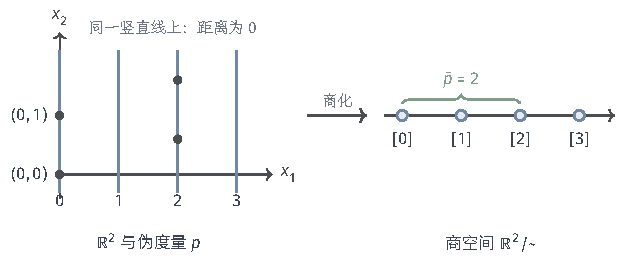
\includegraphics[width=104.916mm]{figures/02-abstract-mathematics/01-metric-and-measure/tikz/c1-pseudometric-quotient/figure.pdf}
  \caption{伪度量$p(\bm x,\bm y)=|x_1-y_1|$与商度量。左侧同一条竖直线上的点（如$(0,0)$与$(0,1)$）相互距离为零，构成一个等价类；右侧每条竖直线成为实轴上的一个点，两类之间的距离是横坐标之差，例如$|2-0|=2$。}
  \label{fig:metric-pseudometric-quotient}
\end{figure}
